\documentclass[12pt]{report}

\usepackage{geometry}
\usepackage[T1]{fontenc}
\usepackage[utf8]{inputenc}
\usepackage[francais]{babel}

\usepackage{graphicx}
\usepackage{lmodern}

\geometry{margin=2cm}


\begin{document}

\thispagestyle{empty}
\noindent
\includegraphics[width=0.25\textwidth]{enseirb-matmeca}

\vspace{\stretch{1}}

\begin{center}
	\Huge{\textbf{Rapport de projet SGBD :}}
	
	\Huge{\textbf{Bandes dessinées}}
\end{center}

\vspace{\stretch{2}}

\begin{tabular}{r@{:~}l}
	\textbf{Auteurs} & \textit{David Bitonneau, Ludovic Hofer, Benoît Ruelle}\\
	\textbf{Encadrants} & \textit{Mme. Allyx Fontaine, M. Sylvain Lombardy,
M. Mohamed Mosbah}\\
\end{tabular}

\vspace{\stretch{1}}

\begin{center}Deuxième année, filière informatique

Date : \today\end{center}

\newpage

\section{Introduction}

re-decrire le sujet en detaillant

\section{Modélisation des données}

Justifier vos choix/hypotheses avec du texte

\subsection{Description du contexte de l'application (entités, associations, règles de gestion)}

-> [Modèle entité-association]

\section{Schéma relationnel :}

\subsection{Passage au relationnel}

\subsection{Contraintes d'intégrité, dépendances fonctionnelles}

\subsection{Schéma relationnel en 3e forme normale}

\noindent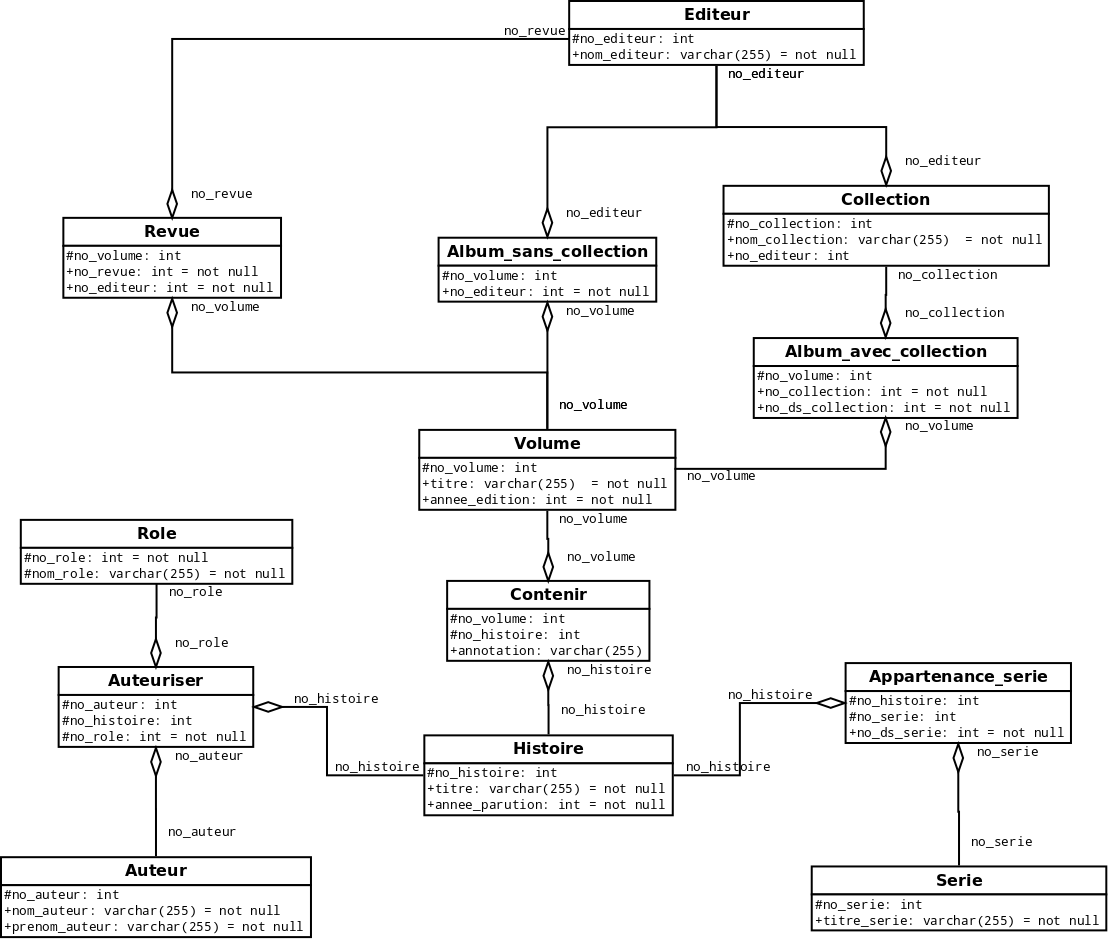
\includegraphics[width=\textwidth]{schema-relation}

\section{Implémentation }
-> choix de MySQL

\subsection{Création de la base de données, en prenant en compte les contraintes d'intégrité (scripts de création, suppression, insertion)}

\subsection{Implémentation des commandes SQL réalisant les opérations retenues}

Lister les requetes importantes

\section{Utilisation :}

\subsection{Description de l'environnement d'exécution}

Decrire l'environnement et l'installation

\subsection{Notice d'utilisation}

\subsection{Description des interfaces éventuelles (Shell, JDBC, PHP, etc.)}

\end{document}
